\documentclass[landscape,final,a1paper,fontscale=0.4]{../baposter/baposter}

\usepackage[american]{babel}
%\usepackage{fixltx2e}
\usepackage{babelbib}
\usepackage[utf8]{inputenc}

\usepackage{calc}
\usepackage{graphicx}
\usepackage{amsmath}
\usepackage{amssymb}
\usepackage{relsize}
\usepackage{multirow}
\usepackage{rotating}
\usepackage{bm}
\usepackage{url}

\usepackage{graphicx}
\usepackage{multicol}

%\usepackage{times}
\usepackage{helvet}
%\usepackage{bookman}
\usepackage{palatino}

\usepackage{floatflt}

\newcommand{\captionfont}{\footnotesize}

\graphicspath{{images/}{../images/}}
\usetikzlibrary{calc}

%%%%%%%%%%%%%%%%%%%%%%%%%%%%%%%%%%%%%%%%%%%%%%%%%%%%%%%%%%%%%%%%%%%%%%%%%%%%%%%%
% Multicol Settings
%%%%%%%%%%%%%%%%%%%%%%%%%%%%%%%%%%%%%%%%%%%%%%%%%%%%%%%%%%%%%%%%%%%%%%%%%%%%%%%%
\setlength{\columnsep}{1.5em}
\setlength{\columnseprule}{0mm}

%%%%%%%%%%%%%%%%%%%%%%%%%%%%%%%%%%%%%%%%%%%%%%%%%%%%%%%%%%%%%%%%%%%%%%%%%%%%%%%%
% Save space in lists. Use this after the opening of the list
%%%%%%%%%%%%%%%%%%%%%%%%%%%%%%%%%%%%%%%%%%%%%%%%%%%%%%%%%%%%%%%%%%%%%%%%%%%%%%%%
\newcommand{\compresslist}{%
\setlength{\itemsep}{1pt}%
\setlength{\parskip}{0pt}%
\setlength{\parsep}{0pt}%
}

%%%%%%%%%%%%%%%%%%%%%%%%%%%%%%%%%%%%%%%%%%%%%%%%%%%%%%%%%%%%%%%%%%%%%%%%%%%%%%
%%% Begin of Document
%%%%%%%%%%%%%%%%%%%%%%%%%%%%%%%%%%%%%%%%%%%%%%%%%%%%%%%%%%%%%%%%%%%%%%%%%%%%%%

\begin{document}

%%%%%%%%%%%%%%%%%%%%%%%%%%%%%%%%%%%%%%%%%%%%%%%%%%%%%%%%%%%%%%%%%%%%%%%%%%%%%%
%%% Here starts the poster
%%%---------------------------------------------------------------------------
%%% Format it to your taste with the options
%%%%%%%%%%%%%%%%%%%%%%%%%%%%%%%%%%%%%%%%%%%%%%%%%%%%%%%%%%%%%%%%%%%%%%%%%%%%%%
% Define some colors

%\definecolor{lightblue}{cmyk}{0.83,0.24,0,0.12}
%\definecolor{lightblue}{rgb}{0.145,0.6666,1}

% HSA-Farben
\definecolor{hsa_himbeerrot}{RGB}{205,0,69}
\definecolor{hsa_reinorange}{RGB}{255,101,0}
\definecolor{hsa_blau}{RGB}{29,96,210}
\definecolor{hsa_hellgrau}{RGB}{161,153,144}
\definecolor{hsa_dunkelgrau}{RGB}{98,98,103}

\begin{poster}%
  % Poster Options
  {
  % Show grid to help with alignment
  grid=false,
  columns=6,
  % Column spacing
  colspacing=1em,
  % Color style
  bgColorOne=white,
  bgColorTwo=hsa_hellgrau,
  borderColor=hsa_reinorange,
  headerColorOne=hsa_reinorange,
  headerColorTwo=hsa_himbeerrot,
  headerFontColor=white,
  boxColorOne=white,
  boxColorTwo=hsa_reinorange,
  % Format of textbox
  %textborder=roundedleft,
  textborder=bars,
  % Format of text header
  eyecatcher=true,
  headerborder=closed,
  headerheight=0.1\textheight,
%  textfont=\sc, An example of changing the text font
  headershape=rectangle,
  headershade=plain,
  headerfont=\Large\bf\sc, %Sans Serif
  textfont={\sf\setlength{\parindent}{1.5em}},
  boxshade=plain,
  %background=shade-tb,
  background=plain,
  linewidth=2pt
  }
  % Eye Catcher
  {
  	    
\includegraphics[height=5em]{images/names.png}
  %\includegraphics[height=5em]{images/graph_occluded.pdf}
  %\includegraphics[height=5em]{images/platzhalter_horizontal}
  } 
  % Title
  {\bf\textsc{Brain Computer Interface}\vspace{0.5em}
  }
  % Subtitle
  {\bf\textsc{Home automation overview}
  		%Überblick über die Grundlagen so wie der Homeautomation} %\vspace{0.5em}
  }
  % University logo
  {% The makebox allows the title to flow into the logo, this is a hack because of the L shaped logo.
    %\includegraphics[height=9.0em]{images/logo}
    
\includegraphics[height=5em]{images/hsa_logo_normal.jpg}
  }	
%%%%%%%%%%%%%%%%%%%%%%%%%%%%%%%%%%%%%%%%%%%%%%%%%%%%%%%%%%%%%%%%%%%%%%%%%%%%%%
%%% Now define the boxes that make up the poster
%%%---------------------------------------------------------------------------
%%% Each box has a name and can be placed absolutely or relatively.
%%% The only inconvenience is that you can only specify a relative position 
%%% towards an already declared box. So if you have a box attached to the 
%%% bottom, one to the top and a third one which should be in between, you 
%%% have to specify the top and bottom boxes before you specify the middle 
%%% box.
%%%%%%%%%%%%%%%%%%%%%%%%%%%%%%%%%%%%%%%%%%%%%%%%%%%%%%%%%%%%%%%%%%%%%%%%%%%%%%

%%%%%%%%%%%%%%%%%%%%%%%%%%%%%%%%%%%%%%%%%%%%%%%%%%%%%%%%%%%%%%%%%%%%%%%%%%%%%%
  \headerbox{Challenge}{name=definition,column=0,span=2,row=0}{
%%%%%%%%%%%%%%%%%%%%%%%%%%%%%%%%%%%%%%%%%%%%%%%%%%%%%%%%%%%%%%%%%%%%%%%%%%%%%%
%\begin{flushleft}
	The main ambition of our project ("Wo issn des Hirn? 2.0") was to improve upon previous efforts to analyze and react to brain activity via brain computer interfaces. This would involve improving the signal quality and classifier accuracy. Additionally, we sought to implement a method to control smart home devices using visual selection via an Android app.
%\end{flushleft}
}
  

%%%%%%%%%%%%%%%%%%%%%%%%%%%%%%%%%%%%%%%%%%%%%%%%%%%%%%%%%%%%%%%%%%%%%%%%%%%%%%
  \headerbox{Smart Home Brain Remote}{name=anlage,column=2,span=2,row=0}{
%%%%%%%%%%%%%%%%%%%%%%%%%%%%%%%%%%%%%%%%%%%%%%%%%%%%%%%%%%%%%%%%%%%%%%%%%%%%%%
%\begin{flushleft}
	
The Smart Home Brain Remote enables users to control various smart home devices using their brain. The application's current stage of development features a menu with three flickering "buttons" (the flickering ensures that the buttons can later be distinguished from one another).  Activating the left or right button allows the user to cycle through the assorted device functions, while activating the middle button will cause the selected function to be executed (examples include "toggle lightbulb", "play music", "stop music", etc.).

To activate a button, the user concentrates on it for a few seconds. A short delay follows, to ensure that the same action is not being activated accidentally. The current setup allows users to control a stream of music from Spotify or manipulate WiFi-controlled sockets in order to turn on lights or other electronic devices. 

	%\vspace{0.25cm}
	\begin{center}
	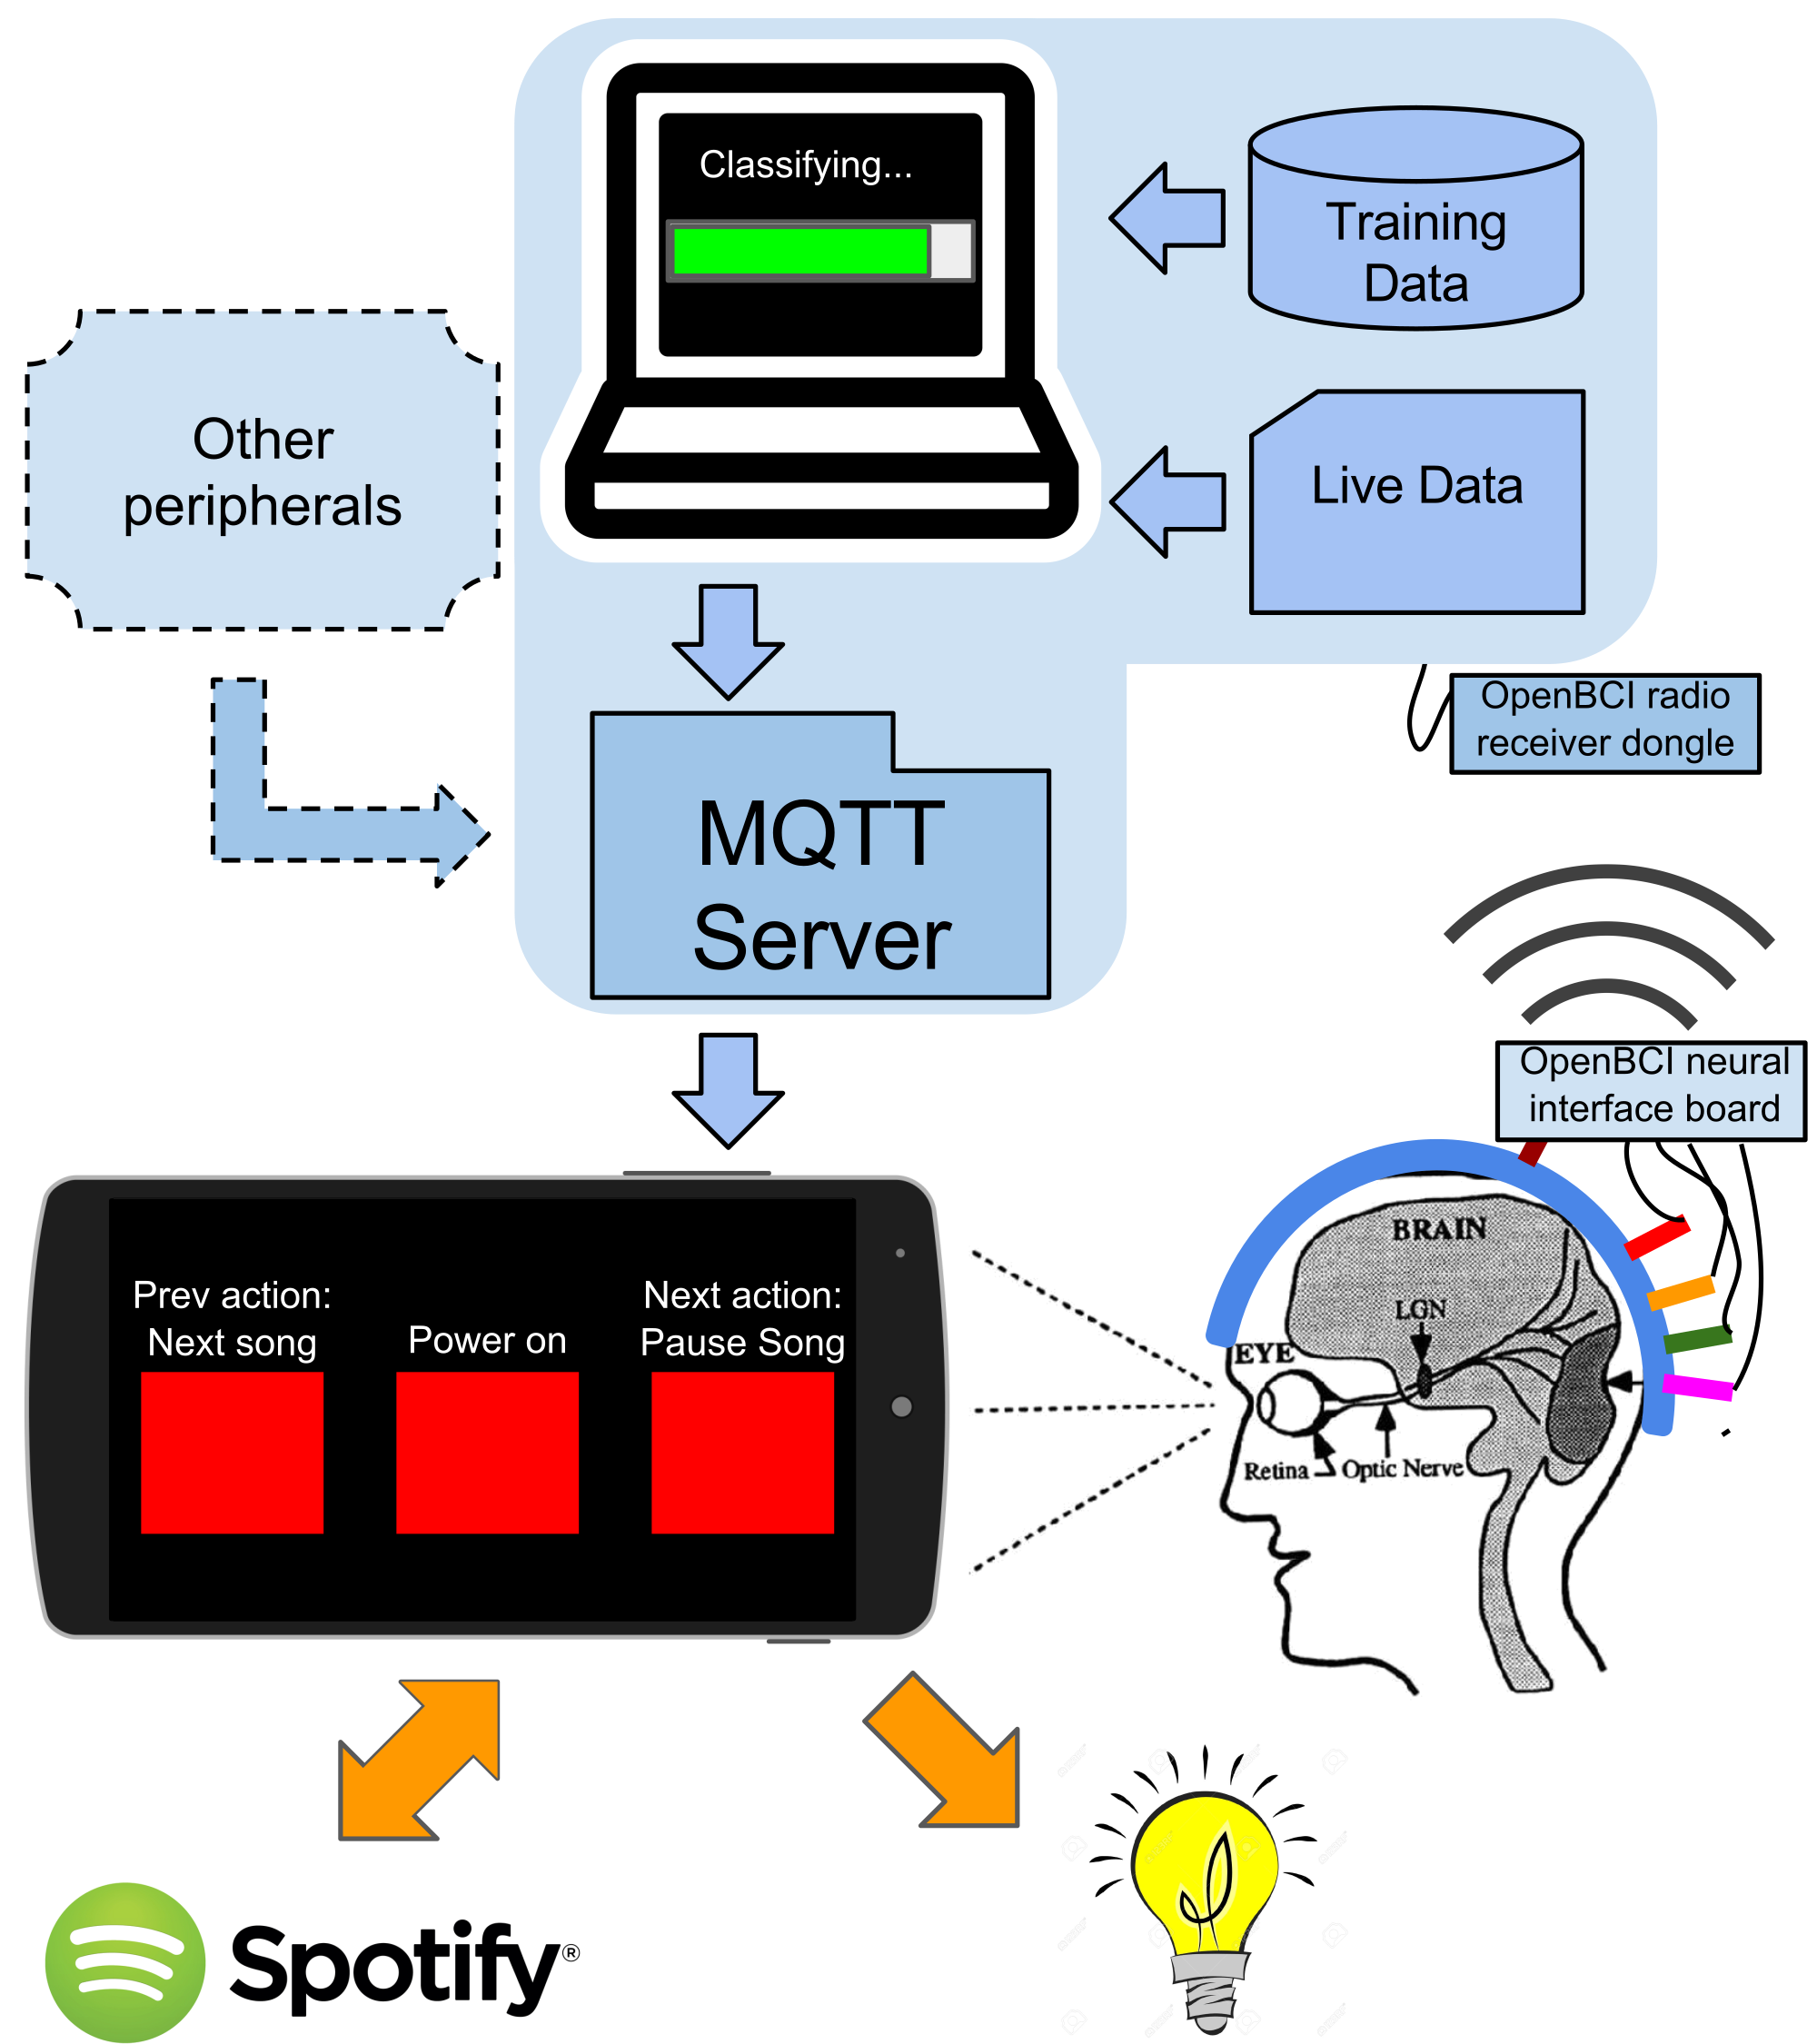
\includegraphics[width=0.95\textwidth]{images/v2.png}
	\end{center}
	
%\end{flushleft}
  }
  
%%%%%%%%%%%%%%%%%%%%%%%%%%%%%%%%%%%%%%%%%%%%%%%%%%%%%%%%%%%%%%%%%%%%%%%%%%%%%%
  \headerbox{Recording of the activities}{name=boards,column=4,span=2,row=0 }{
%%%%%%%%%%%%%%%%%%%%%%%%%%%%%%%%%%%%%%%%%%%%%%%%%%%%%%%%%%%%%%%%%%%%%%%%%%%%%%
%\begin{flushleft}
Our brain computer interface setup uses an arrangement of ten electrodes placed around the visual cortex of the brain. Of these ten electrodes, eight are used to capture brain activity directly, and two act as the noise reduction bias and ground connection. 

 Assuming the electrodes are placed correctly, the Biosensing Board relays the raw electrode signals to the computer, where signal processing takes place. In order to ensure flawless signal acquisition, the electrodes must remain perfectly stationary during the recording phase, facilitated by our custom-made electrode holders, which are placed into a flexible EEG cap. Another source of errors during the recording phase is the interference of WiFi-enabled devices and other sources of EM noise. Lastly, the user whose brain signals are being analyzed should be a in a relaxed state of mind.
	\begin{center}
 	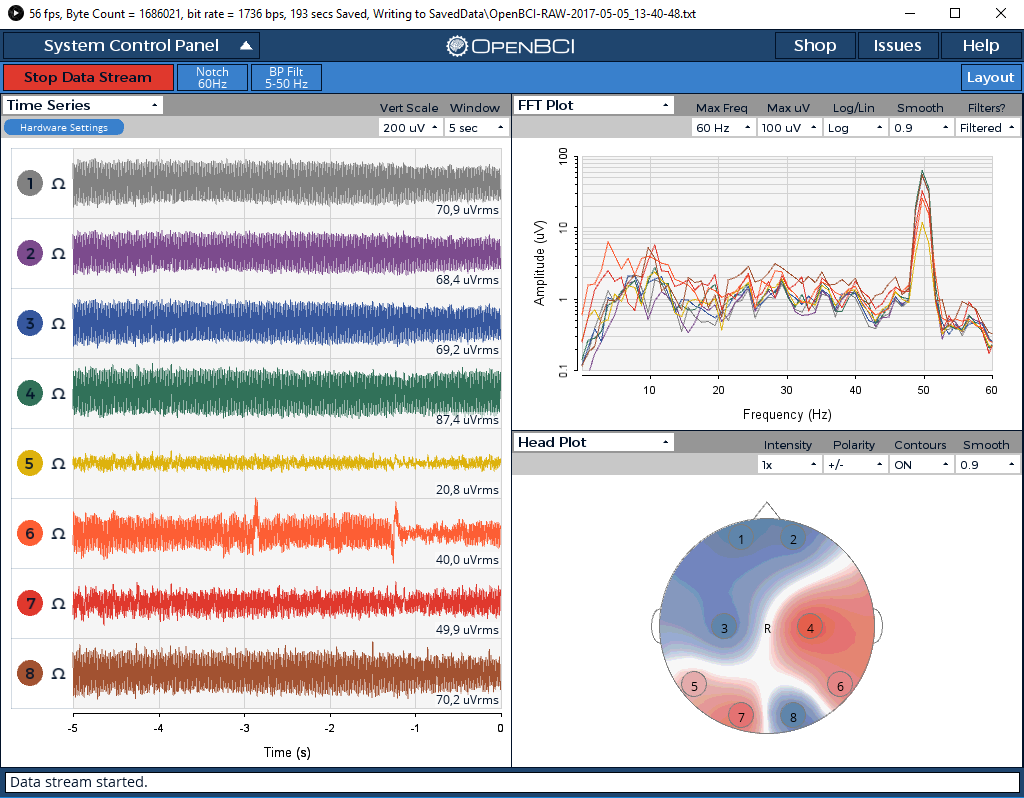
\includegraphics[scale=0.28]{images/OpenBCI.png}
	\end{center}

%    \end{flushleft}
  }

%%%%%%%%%%%%%%%%%%%%%%%%%%%%%%%%%%%%%%%%%%%%%%%%%%%%%%%%%%%%%%%%%%%%%%%%%%%%%%  
  \headerbox{References}{name=projhsa,column=4,span=2,row=0.66}{
%%%%%%%%%%%%%%%%%%%%%%%%%%%%%%%%%%%%%%%%%%%%%%%%%%%%%%%%%%%%%%%%%%%%%%%%%%%%%%
 %\begin{flushleft}
 
 \smaller
 \bibliographystyle{ieee}
 \renewcommand{\section}[2]{\vskip 0.05em}
 \begin{thebibliography}{1}\itemsep=-0.01em
 	
 	\setlength{\baselineskip}{0.4em}
 	\bibitem{SSVEP}
 	Robert Prueckl and Christoph Guger , “A Brain-Computer Interface Based on Steady State Visual Evoked Potentials for Controlling a Robot” [Online]. Available: \url{www.gtec.at/content/download/1822/11397/version/2/}. [Accessed: 19-June-2017].
 	
 	\setlength{\baselineskip}{0.4em}
 	\bibitem{motor imaginary}
 	Maitreyee Wairagkar” Brain Embodiment Lab, School of Systems Engineering, University of Reading, Reading, U.K.[Online]. Available: \url {https://www.bcur.org/journals/index.php/BCURProc/article/download/6/5}. [Accessed: 19-June-2017]
 	
 	\setlength{\baselineskip}{0.4em}
 	\bibitem{svm}
 	Yuanqing Li, Cuntai Guan, Huiqi Li, Zhengyang Chin “A self-training semi-supervised SVM algorithm and its application
 	in an EEG-based brain computer interface speller system” Institute for Inforcomm Research, Heng Mui Keng Terrace, 21, Singapore 119613, Singapore.[Online]. Available: \url{http://www.sciencedirect.com/science/article/pii/S016786550800055X}. [Accessed: 19-June-2017]
 	
 \end{thebibliography}
 %\vspace{0.3em}
 %\end{flushleft}
}

%%%%%%%%%%%%%%%%%%%%%%%%%%%%%%%%%%%%%%%%%%%%%%%%%%%%%%%%%%%%%%%%%%%%%%%%%%%%%%%
 \headerbox{State of the Art}{name=references,column=0,span=2,below=definition}{
%%%%%%%%%%%%%%%%%%%%%%%%%%%%%%%%%%%%%%%%%%%%%%%%%%%%%%%%%%%%%%%%%%%%%%%%%%%%%%%

This project is not the first attempt at creating an interface between the brain and the computer. One of many such applications is a Steady State Visually Evoked Potential (SSVEP) speller, which can detect the character that a user wishes to select by displaying each letter of the alphabet with a blinking background and then measuring the electrical activity of the visual cortex of the brain. \cite{SSVEP}

A different brain computer interface methodology involves measuring the activity in the motor cortex of the brain  that happens as a result of moving, or envisioning moving, one's arms and legs \cite{motor imaginary}. 

Regardless of the application, recording brain activity entails placing electrodes on specific locations on the subject's head and then measuring the electrical resistance between pairs of electrodes. This processed signal can then be analyzed in a number of ways.

A Naive Bayes Classifier, for example, calculates the probabilities of the portion of a signal falling into each of several categories, based on previous training data. A Support Vector Machine (SVM) classifier attempts to divide the training data into two or more groups by means of reducing a multi-dimensional array, and outputting the group most similar to the input data. \cite{svm}

	\begin{center}
		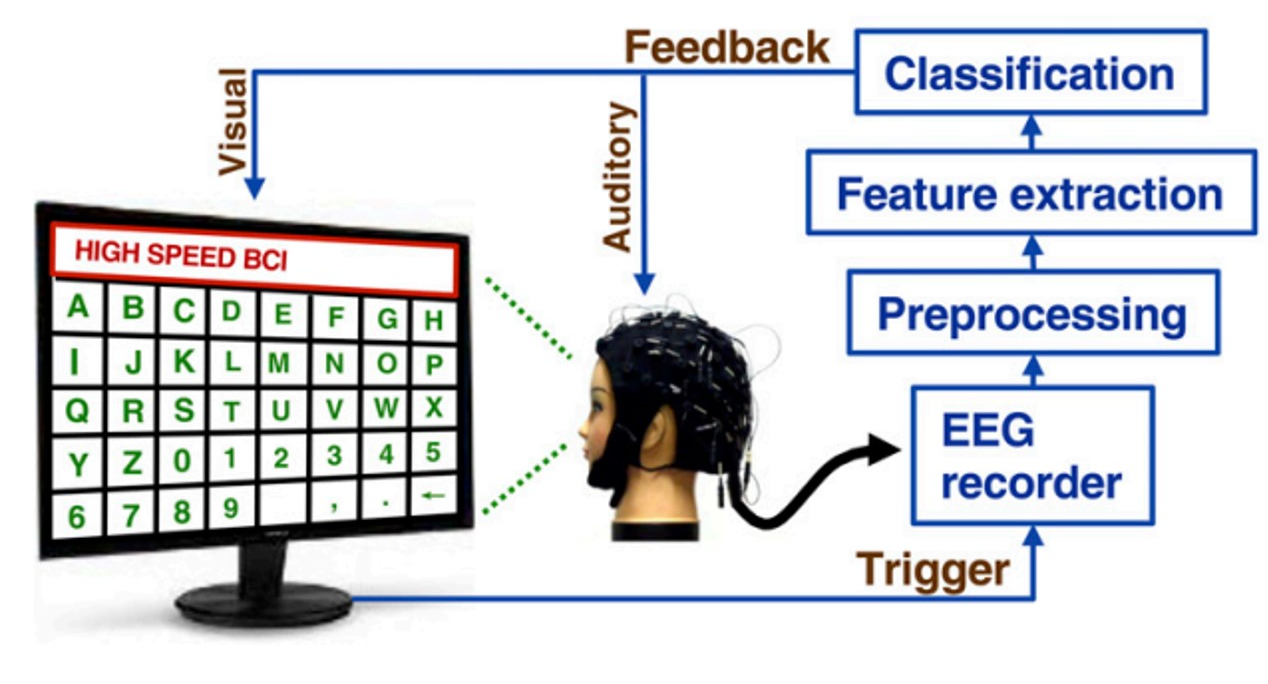
\includegraphics[scale=0.3]{images/ssvep_example.png}\newline
		SSVEP Speller (sciencemission.com)
	\end{center}
   
}
    
    
  
    

\end{poster}

\end{document}

